\documentclass{beamer}
\usetheme{Madrid}
\usecolortheme{default}

% Packages
\usepackage{graphicx}
\usepackage{booktabs}
\usepackage{tikz}
\usepackage{amsmath}

% Title and authors
\title{\textbf{Evaluating Small Language Models for News Summarization}}
\subtitle{Implications and Factors Influencing Performance}
\author{Aman Agarwal \and Nakul Siwach \and Himanshu Shivhare}
\institute{International Institute of Information Technology, Bangalore}
\date{\today}

% Custom colors
\definecolor{iiitblue}{RGB}{0,51,102}
\definecolor{successgreen}{RGB}{46,204,113}
\definecolor{warningred}{RGB}{231,76,60}

% Remove footer
\setbeamertemplate{footline}{}
\setbeamertemplate{navigation symbols}{}

\begin{document}

% Title slide
\frame{\titlepage}

% Outline
\begin{frame}{Outline}
\tableofcontents
\end{frame}

\section{Introduction}

\begin{frame}{Motivation}
\begin{itemize}
    \item \textbf{Problem}: Small Language Models (SLMs) are gaining importance for resource-constrained environments
    \item \textbf{Challenge}: Which learning approach is best for SLMs in news summarization?
    \begin{itemize}
        \item Zero-shot?
        \item Few-shot?
        \item Full fine-tuning?
        \item Parameter-efficient fine-tuning (LoRA)?
    \end{itemize}
    \item \textbf{Gap}: Conventional wisdom says "always fine-tune" - but is this true?
\end{itemize}

\vspace{0.5cm}
\begin{alertblock}{Key Question}
Does the optimal approach depend on model architecture?
\end{alertblock}
\end{frame}

\begin{frame}{Research Questions}
\begin{enumerate}
    \item \textbf{RQ1}: How do different learning approaches affect performance across SLM architectures?
    
    \item \textbf{RQ2}: Does fine-tuning improve or degrade instruction-tuned models?
    
    \item \textbf{RQ3}: What are the minimum model size requirements for effective LoRA fine-tuning?
    
    \item \textbf{RQ4}: How do performance-efficiency trade-offs vary across approaches?
\end{enumerate}
\end{frame}

\section{Methodology}

\begin{frame}{Experimental Setup}
\begin{columns}
\column{0.5\textwidth}
\textbf{Models Evaluated (3)}
\begin{itemize}
    \item FLAN-T5-Small (80M)
    \item FLAN-T5-Base (250M)
    \item BART-Base (140M)
\end{itemize}

\vspace{0.3cm}
\textbf{Learning Approaches (4)}
\begin{itemize}
    \item Zero-shot
    \item Few-shot (3 examples)
    \item Full fine-tuning
    \item LoRA fine-tuning
\end{itemize}

\column{0.5\textwidth}
\textbf{Dataset}
\begin{itemize}
    \item CNN/DailyMail
    \item 1,000 training samples
    \item 100 test samples
\end{itemize}

\vspace{0.3cm}
\textbf{Metrics}
\begin{itemize}
    \item ROUGE-1, ROUGE-2, ROUGE-L
    \item BERTScore
\end{itemize}

\vspace{0.3cm}
\textbf{Total Experiments}
\begin{center}
\Large{3 models × 4 approaches = \textbf{12 evaluations}}
\end{center}
\end{columns}
\end{frame}

\begin{frame}{Model Architectures}
\begin{table}
\centering
\begin{tabular}{lc}
\toprule
\textbf{Model} & \textbf{Parameters} \\
\midrule
FLAN-T5-Small & 80M \\
FLAN-T5-Base & 250M \\
BART-Base & 140M \\
\bottomrule
\end{tabular}
\end{table}

\vspace{0.5cm}
\textbf{Key Difference}:
\begin{itemize}
    \item \textcolor{blue}{\textbf{FLAN-T5}}: Pre-trained to follow instructions (zero-shot capable)
    \item \textcolor{orange}{\textbf{BART}}: Pre-trained for text generation (needs task-specific training)
\end{itemize}
\end{frame}

\section{Results}

\begin{frame}{Overall Performance Comparison}
\begin{figure}
\centering
\includegraphics[width=0.95\textwidth]{figure1_performance_comparison.pdf}
\end{figure}

\begin{alertblock}{Key Observation}
Different models perform best with different approaches!
\end{alertblock}
\end{frame}

\begin{frame}{Top 3 Results}
\begin{table}
\centering
\begin{tabular}{clcc}
\toprule
\textbf{Rank} & \textbf{Model + Approach} & \textbf{ROUGE-1} & \textbf{BERTScore} \\
\midrule
🥇 & BART-Base Full FT & \textbf{33.06\%} & \textbf{87.55\%} \\
🥈 & FLAN-T5-Base Zero-shot & \textbf{32.50\%} & \textbf{87.19\%} \\
🥉 & FLAN-T5-Small Few-shot & \textbf{32.29\%} & \textbf{87.68\%} \\
\bottomrule
\end{tabular}
\end{table}

\vspace{0.3cm}
\begin{block}{Surprising Finding}
FLAN-T5-Base zero-shot (no training!) is only 0.56 pp behind the best result!
\end{block}
\end{frame}

\begin{frame}{Results by Model}
\begin{table}
\centering
\small
\begin{tabular}{lcccc}
\toprule
\textbf{Model} & \textbf{ZS} & \textbf{FS} & \textbf{FFT} & \textbf{LFT} \\
\midrule
FLAN-T5-Small & 29.56 & \textcolor{successgreen}{\textbf{32.29}} & 28.39 & 26.16 \\
FLAN-T5-Base & \textcolor{successgreen}{\textbf{32.50}} & 27.63 & 28.39 & 29.75 \\
BART-Base & 30.74 & \textcolor{warningred}{11.99} & \textcolor{successgreen}{\textbf{33.06}} & 31.13 \\
\bottomrule
\end{tabular}
\caption{ROUGE-1 F1 scores (\%). ZS: Zero-shot, FS: Few-shot, FFT: Full FT, LFT: LoRA FT}
\end{table}

\vspace{0.3cm}
\textbf{Pattern}:
\begin{itemize}
    \item \textcolor{blue}{FLAN-T5}: Best with zero-shot/few-shot
    \item \textcolor{orange}{BART}: Best with fine-tuning
\end{itemize}
\end{frame}

\section{Key Findings}

\begin{frame}{Finding 1: Catastrophic Forgetting}
\begin{figure}
\centering
\includegraphics[width=0.85\textwidth]{figure3_catastrophic_forgetting.pdf}
\end{figure}

\begin{alertblock}{Critical Discovery}
Fine-tuning \textbf{degrades} instruction-tuned models (FLAN-T5)!
\end{alertblock}
\end{frame}

\begin{frame}{Finding 1: Catastrophic Forgetting (Details)}
\textbf{FLAN-T5 Models - Fine-tuning Makes Them WORSE!}

\begin{table}
\centering
\begin{tabular}{lccc}
\toprule
\textbf{Model} & \textbf{Zero-shot} & \textbf{Fine-tuned} & \textbf{Change} \\
\midrule
FLAN-T5-Small & 29.56\% & 28.39\% & \textcolor{warningred}{-1.17 pp} \\
FLAN-T5-Base & 32.50\% & 28.39\% & \textcolor{warningred}{-4.11 pp} \\
\midrule
BART-Base & 30.74\% & 33.06\% & \textcolor{successgreen}{+2.32 pp} \\
\bottomrule
\end{tabular}
\end{table}

\vspace{0.3cm}
\textbf{Explanation}:
\begin{itemize}
    \item Instruction-tuned models learn general instruction-following
    \item Task-specific fine-tuning overwrites this capability
    \item Result: Performance degrades despite more training!
\end{itemize}
\end{frame}

\begin{frame}{Finding 2: LoRA Size Thresholds}
\begin{figure}
\centering
\includegraphics[width=0.85\textwidth]{figure2_lora_effectiveness.pdf}
\end{figure}

\begin{block}{Threshold Discovery}
LoRA needs sufficient model size: 250M+ for instruction-tuned, 140M+ for generation-focused
\end{block}
\end{frame}

\begin{frame}{Finding 2: LoRA Size Thresholds (Details)}
\textbf{LoRA Performance vs. Full Fine-tuning}

\begin{table}
\centering
\begin{tabular}{lcc}
\toprule
\textbf{Model} & \textbf{Size} & \textbf{LoRA vs FFT} \\
\midrule
FLAN-T5-Small & 80M & \textcolor{warningred}{-2.23 pp} \\
BART-Base & 140M & \textcolor{orange}{-1.93 pp} \\
FLAN-T5-Base & 250M & \textcolor{successgreen}{+1.36 pp} \\
\bottomrule
\end{tabular}
\end{table}

\vspace{0.3cm}
\textbf{Key Insights}:
\begin{itemize}
    \item Smaller models (80M): LoRA fails
    \item Medium models (140M+): LoRA works for generation-focused
    \item Larger models (250M+): LoRA works well for instruction-tuned
    \item LoRA can even \textbf{outperform} full fine-tuning!
\end{itemize}
\end{frame}

\begin{frame}{Finding 3: Zero-shot Superiority}
\begin{figure}
\centering
\includegraphics[width=0.7\textwidth]{figure4_approach_averages.pdf}
\end{figure}

\begin{alertblock}{Surprising Result}
Zero-shot achieves \textbf{highest average} performance across all models!
\end{alertblock}
\end{frame}

\begin{frame}{Finding 3: Zero-shot Superiority (Details)}
\textbf{Average Performance Across All Models}

\begin{table}
\centering
\begin{tabular}{lcc}
\toprule
\textbf{Approach} & \textbf{Avg ROUGE-1} & \textbf{Rank} \\
\midrule
\textcolor{successgreen}{\textbf{Zero-shot}} & \textcolor{successgreen}{\textbf{30.93\%}} & \textcolor{successgreen}{\textbf{1st}} \\
Full Fine-tuning & 29.95\% & 2nd \\
LoRA Fine-tuning & 29.01\% & 3rd \\
Few-shot & 23.97\% & 4th \\
\bottomrule
\end{tabular}
\end{table}

\vspace{0.3cm}
\textbf{Implication}:
\begin{itemize}
    \item Training is \textbf{not always beneficial}!
    \item Zero-shot should be the baseline, not an afterthought
    \item Challenges conventional "always fine-tune" assumption
\end{itemize}
\end{frame}

\begin{frame}{Finding 4: Few-shot Unreliability}
\textbf{Few-shot Performance is Highly Variable}

\begin{table}
\centering
\begin{tabular}{lcc}
\toprule
\textbf{Model} & \textbf{Few-shot} & \textbf{vs Zero-shot} \\
\midrule
FLAN-T5-Small & \textcolor{successgreen}{32.29\%} & \textcolor{successgreen}{+2.73 pp ✓} \\
FLAN-T5-Base & \textcolor{orange}{27.63\%} & \textcolor{orange}{-4.87 pp} \\
BART-Base & \textcolor{warningred}{11.99\%} & \textcolor{warningred}{-18.75 pp ✗✗✗} \\
\midrule
\textbf{Range} & \multicolumn{2}{c}{\textbf{20.3 percentage points!}} \\
\bottomrule
\end{tabular}
\end{table}

\vspace{0.3cm}
\begin{alertblock}{Warning}
Few-shot is too unpredictable for production systems!
\end{alertblock}
\end{frame}

\begin{frame}{Finding 5: Efficiency-Performance Trade-off}
\begin{figure}
\centering
\includegraphics[width=0.85\textwidth]{figure5_efficiency_tradeoff.pdf}
\end{figure}

\begin{block}{LoRA Sweet Spot}
LoRA achieves 94\% of full FT performance with 50\% less time!
\end{block}
\end{frame}

\begin{frame}{Finding 5: LoRA Efficiency Benefits}
\textbf{LoRA vs. Full Fine-tuning for BART-Base}

\begin{table}
\centering
\small
\begin{tabular}{lccc}
\toprule
\textbf{Metric} & \textbf{Full FT} & \textbf{LoRA FT} & \textbf{Savings} \\
\midrule
ROUGE-1 & 33.06\% & 31.13\% & -1.93 pp (6\%) \\
Training Time & 45-60 min & 20-30 min & \textcolor{successgreen}{50\%} \\
Parameters Trained & 140M & 0.5M & \textcolor{successgreen}{99.6\%} \\
Memory & 10-12 GB & 6-8 GB & \textcolor{successgreen}{40\%} \\
\bottomrule
\end{tabular}
\end{table}

\vspace{0.3cm}
\textbf{Trade-off}: Lose 1.93 pp performance, gain massive efficiency!

\textbf{Verdict}: Excellent for practical deployment!
\end{frame}

\section{Practical Recommendations}

\begin{frame}{Architecture-Approach Matching}
\begin{columns}
\column{0.5\textwidth}
\textbf{Instruction-Tuned Models}\\
(FLAN-T5, T0, etc.)

\vspace{0.3cm}
\textcolor{successgreen}{\textbf{✓ Recommended}}:
\begin{itemize}
    \item Zero-shot
    \item Few-shot (if validated)
    \item LoRA FT (250M+ only)
\end{itemize}

\vspace{0.3cm}
\textcolor{warningred}{\textbf{✗ Not Recommended}}:
\begin{itemize}
    \item Full fine-tuning
    \item LoRA FT (<250M)
\end{itemize}

\column{0.5\textwidth}
\textbf{Generation-Focused Models}\\
(BART, Pegasus, etc.)

\vspace{0.3cm}
\textcolor{successgreen}{\textbf{✓ Recommended}}:
\begin{itemize}
    \item Full fine-tuning
    \item LoRA fine-tuning
    \item Zero-shot (no data)
\end{itemize}

\vspace{0.3cm}
\textcolor{warningred}{\textbf{✗ Not Recommended}}:
\begin{itemize}
    \item Few-shot learning
\end{itemize}
\end{columns}
\end{frame}

\begin{frame}{Decision Framework}
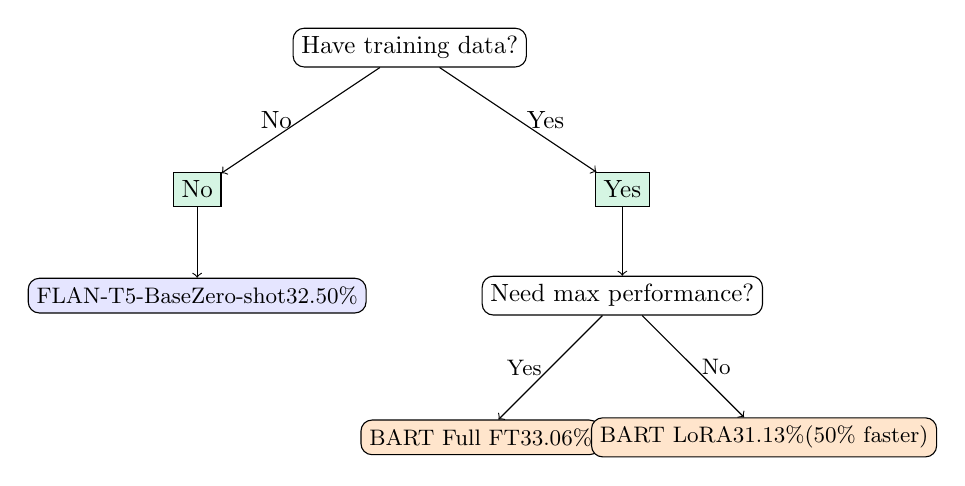
\begin{tikzpicture}[scale=0.9, transform shape]
% Decision tree
\node[draw, rectangle, rounded corners] (start) at (0,0) {Have training data?};

\node[draw, rectangle, fill=successgreen!20] (no) at (-3,-2) {No};
\node[draw, rectangle, fill=successgreen!20] (yes) at (3,-2) {Yes};

\draw[->] (start) -- (no) node[midway, left] {No};
\draw[->] (start) -- (yes) node[midway, right] {Yes};

\node[draw, rectangle, rounded corners, fill=blue!10] (flan) at (-3,-3.5) 
    {\small FLAN-T5-Base\\Zero-shot\\32.50\%};
\draw[->] (no) -- (flan);

\node[draw, rectangle, rounded corners] (need) at (3,-3.5) {Need max performance?};
\draw[->] (yes) -- (need);

\node[draw, rectangle, rounded corners, fill=orange!20] (fullft) at (1,-5.5) 
    {\small BART Full FT\\33.06\%};
\node[draw, rectangle, rounded corners, fill=orange!20] (lora) at (5,-5.5) 
    {\small BART LoRA\\31.13\%\\(50\% faster)};

\draw[->] (need) -- (fullft) node[midway, left] {\small Yes};
\draw[->] (need) -- (lora) node[midway, right] {\small No};
\end{tikzpicture}
\end{frame}

\begin{frame}{Deployment Scenarios}
\begin{table}
\centering
\small
\begin{tabular}{lll}
\toprule
\textbf{Scenario} & \textbf{Best Choice} & \textbf{ROUGE-1} \\
\midrule
No training data & FLAN-T5-Base Zero-shot & 32.50\% \\
Max performance & BART-Base Full FT & 33.06\% \\
Efficiency focus & BART-Base LoRA FT & 31.13\% \\
Limited compute & FLAN-T5-Small Few-shot & 32.29\% \\
Multiple tasks & FLAN-T5-Base Zero-shot & 32.50\% \\
\bottomrule
\end{tabular}
\end{table}

\vspace{0.3cm}
\begin{block}{Key Message}
Match approach to your constraints, not conventional wisdom!
\end{block}
\end{frame}

\section{Contributions}

\begin{frame}{Research Contributions}
\begin{enumerate}
    \item \textbf{Catastrophic Forgetting Discovery}
    \begin{itemize}
        \item First systematic demonstration in instruction-tuned models
        \item Challenges "always fine-tune" assumption
    \end{itemize}
    
    \item \textbf{LoRA Size Thresholds}
    \begin{itemize}
        \item Identified minimum requirements: 250M+ (instruction), 140M+ (generation)
        \item Architecture-dependent success criteria
    \end{itemize}
    
    \item \textbf{Architecture-Approach Matching Framework}
    \begin{itemize}
        \item Clear guidelines for approach selection
        \item Evidence-based deployment recommendations
    \end{itemize}
    
    \item \textbf{Zero-shot Superiority Evidence}
    \begin{itemize}
        \item Highest average performance (30.93\%)
        \item Training not always beneficial
    \end{itemize}
\end{enumerate}
\end{frame}

\begin{frame}{Contributions (cont.)}
\begin{enumerate}
    \setcounter{enumi}{4}
    \item \textbf{Few-shot Unreliability Documentation}
    \begin{itemize}
        \item 20.3 pp performance range
        \item Not suitable for production
    \end{itemize}
    
    \item \textbf{Efficiency-Performance Quantification}
    \begin{itemize}
        \item LoRA: 94\% performance, 50\% time
        \item Clear trade-off analysis
    \end{itemize}
\end{enumerate}

\vspace{0.5cm}
\begin{block}{Impact}
Provides evidence-based guidelines that challenge conventional assumptions and enable better deployment decisions
\end{block}
\end{frame}

\section{Conclusion}

\begin{frame}{Key Takeaways}
\begin{enumerate}
    \item \textbf{Architecture determines optimal approach}
    \begin{itemize}
        \item Instruction-tuned → zero-shot/few-shot
        \item Generation-focused → fine-tuning
    \end{itemize}
    
    \item \textbf{Fine-tuning can hurt instruction-tuned models}
    \begin{itemize}
        \item FLAN-T5-Base: 32.50\% (zero) → 28.39\% (fine-tuned)
    \end{itemize}
    
    \item \textbf{LoRA needs sufficient size}
    \begin{itemize}
        \item Fails at 80M, works at 140M+
    \end{itemize}
    
    \item \textbf{Zero-shot often best}
    \begin{itemize}
        \item Highest average: 30.93\%
    \end{itemize}
    
    \item \textbf{Few-shot unreliable}
    \begin{itemize}
        \item Range: 11.99\% - 32.29\%
    \end{itemize}
\end{enumerate}
\end{frame}

\begin{frame}{Future Work}
\begin{itemize}
    \item \textbf{Expand model coverage}
    \begin{itemize}
        \item Test decoder-only models (GPT-style, Llama)
        \item Evaluate at different size points (100M, 150M, 200M)
    \end{itemize}
    
    \item \textbf{Mitigate catastrophic forgetting}
    \begin{itemize}
        \item Develop adaptive fine-tuning methods
        \item Test regularization approaches
    \end{itemize}
    
    \item \textbf{Optimize LoRA configuration}
    \begin{itemize}
        \item Model-specific hyperparameter tuning
        \item Different rank selections
    \end{itemize}
    
    \item \textbf{Real-world deployment studies}
    \begin{itemize}
        \item Edge device evaluation
        \item User preference studies
    \end{itemize}
\end{itemize}
\end{frame}

\begin{frame}{Summary}
\begin{center}
\Large{\textbf{Main Message}}
\end{center}

\begin{alertblock}{}
\centering
\large
The optimal learning approach depends on model architecture, not size alone.

\vspace{0.3cm}
Match approach to architecture for best results!
\end{alertblock}

\vspace{0.5cm}
\begin{columns}
\column{0.5\textwidth}
\textbf{Best Overall}:\\
BART-Base Full FT\\
33.06\% ROUGE-1

\column{0.5\textwidth}
\textbf{Best Without Training}:\\
FLAN-T5-Base Zero-shot\\
32.50\% ROUGE-1
\end{columns}
\end{frame}

\begin{frame}[standout]
\centering
\Huge{\textbf{Thank You!}}

\vspace{1cm}
\Large{Questions?}

\vspace{1cm}
\normalsize
Aman Agarwal, Nakul Siwach, Himanshu Shivhare\\
International Institute of Information Technology, Bangalore
\end{frame}

\end{document}

